\documentclass[aspectratio=169]{beamer}
\usetheme{Madrid}
\usecolortheme{default}

\usepackage{amsmath, amsfonts, amssymb}
\usepackage{tikz}
\usetikzlibrary{arrows.meta, calc, decorations.pathreplacing, patterns}
\usepackage{pgfplots}
\pgfplotsset{compat=1.18}

\title{Smoothing Splines}
\subtitle{Balancing Fit and Smoothness}
\author{CSE255 - Scalable Data Analysis}
\date{\today}

\begin{document}

\frame{\titlepage}

\begin{frame}{Motivation}
\begin{itemize}
    \item Given data points $(x_i, y_i)$ for $i = 1, \ldots, n$, we want to estimate a smooth function $f(x)$
    \item \textbf{Problem}: Interpolation fits exactly but may be too wiggly
    \item \textbf{Solution}: Smoothing splines balance fit quality with smoothness
    \item Trade-off: Better fit vs. smoother curve
\end{itemize}

\begin{block}{Key Idea}
Find $f$ that minimizes both the residual sum of squares and a roughness penalty
\end{block}
\end{frame}

\begin{frame}{The Smoothing Spline Problem}
Given data $(x_1, y_1), \ldots, (x_n, y_n)$ with $x_1 < x_2 < \cdots < x_n$:

\[
\min_{f} \quad \sum_{i=1}^{n} (y_i - f(x_i))^2 + \lambda \int_{x_1}^{x_n} [f''(t)]^2 \, dt
\]

\begin{itemize}
    \item \textbf{First term}: Residual sum of squares (measures fit quality)
    \item \textbf{Second term}: Roughness penalty (measures smoothness)
    \item \textbf{$\lambda$}: Smoothing parameter (controls trade-off)
    \begin{itemize}
        \item $\lambda = 0$: Interpolation (perfect fit, may be wiggly)
        \item $\lambda \to \infty$: Linear regression (smooth but may not fit well)
    \end{itemize}
\end{itemize}
\end{frame}

\begin{frame}{Natural Cubic Splines}
The solution to the smoothing spline problem is a \textbf{natural cubic spline}:

\begin{block}{Definition}
A function $f$ is a natural cubic spline with knots at $x_1, \ldots, x_n$ if:
\begin{enumerate}
    \item $f$ is a cubic polynomial on each interval $[x_i, x_{i+1}]$
    \item $f$ is twice continuously differentiable at the knots
    \item $f''(x_1) = f''(x_n) = 0$ (natural boundary conditions)
\end{enumerate}
\end{block}

\begin{itemize}
    \item Natural cubic splines have $n$ degrees of freedom
    \item They provide the smoothest interpolant (minimum curvature)
    \item The solution can be computed efficiently using basis functions
\end{itemize}
\end{frame}

\begin{frame}{Basis Representation}
Any natural cubic spline can be written as:

\[
f(x) = \sum_{j=1}^{n} N_j(x) \theta_j
\]

where $N_j(x)$ are \textbf{natural cubic spline basis functions} (B-splines).

\begin{block}{Matrix Form}
\[
\mathbf{f} = \mathbf{N} \boldsymbol{\theta}
\]
where:
\begin{itemize}
    \item $\mathbf{f} = [f(x_1), \ldots, f(x_n)]^\top$
    \item $\mathbf{N}$ is the $n \times n$ basis matrix: $N_{ij} = N_j(x_i)$
    \item $\boldsymbol{\theta} = [\theta_1, \ldots, \theta_n]^\top$ are coefficients
\end{itemize}
\end{block}
\end{frame}

\begin{frame}{Penalized Least Squares Solution}
The smoothing spline problem becomes:

\[
\min_{\boldsymbol{\theta}} \quad \|\mathbf{y} - \mathbf{N}\boldsymbol{\theta}\|^2 + \lambda \boldsymbol{\theta}^\top \boldsymbol{\Omega} \boldsymbol{\theta}
\]

where $\boldsymbol{\Omega}$ is the penalty matrix with entries:
\[
\Omega_{ij} = \int_{x_1}^{x_n} N_i''(t) N_j''(t) \, dt
\]

\begin{block}{Solution}
\[
\hat{\boldsymbol{\theta}} = (\mathbf{N}^\top \mathbf{N} + \lambda \boldsymbol{\Omega})^{-1} \mathbf{N}^\top \mathbf{y}
\]

\[
\hat{\mathbf{f}} = \mathbf{N}(\mathbf{N}^\top \mathbf{N} + \lambda \boldsymbol{\Omega})^{-1} \mathbf{N}^\top \mathbf{y} = \mathbf{S}_\lambda \mathbf{y}
\]

where $\mathbf{S}_\lambda$ is the \textbf{smoothing matrix} (hat matrix).
\end{block}
\end{frame}

\begin{frame}{Effective Degrees of Freedom}
The smoothing matrix $\mathbf{S}_\lambda$ has trace:

\[
\text{df}_\lambda = \text{tr}(\mathbf{S}_\lambda)
\]

\begin{itemize}
    \item Measures the effective number of parameters
    \item $\text{df}_\lambda = n$ when $\lambda = 0$ (interpolation)
    \item $\text{df}_\lambda = 2$ when $\lambda \to \infty$ (linear fit)
    \item Often easier to specify $\text{df}_\lambda$ than $\lambda$ directly
\end{itemize}

\begin{block}{Relationship}
\[
\text{df}_\lambda = \sum_{i=1}^{n} \frac{1}{1 + \lambda d_i}
\]
where $d_i$ are eigenvalues of $\boldsymbol{\Omega}$ relative to $\mathbf{N}^\top \mathbf{N}$
\end{block}
\end{frame}

\begin{frame}{Effect of Smoothing Parameter}
\centering
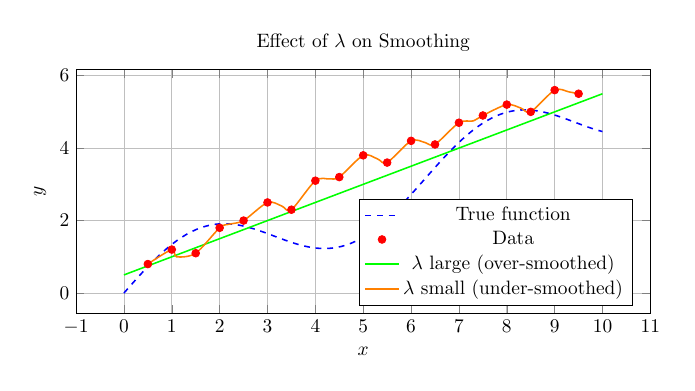
\begin{tikzpicture}[scale=0.7]
    % Generate some noisy data
    \begin{axis}[
        width=12cm,
        height=6cm,
        xlabel={$x$},
        ylabel={$y$},
        title={Effect of $\lambda$ on Smoothing},
        legend pos=south east,
        grid=major
    ]
    % True function (sine wave)
    \addplot[domain=0:10, samples=100, thick, blue, dashed] {sin(deg(x)) + 0.5*x};
    \addlegendentry{True function}
    
    % Data points
    \addplot[only marks, mark=*, mark size=2pt, red] coordinates {
        (0.5, 0.8) (1.0, 1.2) (1.5, 1.1) (2.0, 1.8) (2.5, 2.0)
        (3.0, 2.5) (3.5, 2.3) (4.0, 3.1) (4.5, 3.2) (5.0, 3.8)
        (5.5, 3.6) (6.0, 4.2) (6.5, 4.1) (7.0, 4.7) (7.5, 4.9)
        (8.0, 5.2) (8.5, 5.0) (9.0, 5.6) (9.5, 5.5)
    };
    \addlegendentry{Data}
    
    % Over-smoothed (lambda large)
    \addplot[domain=0:10, samples=100, thick, green] {0.5*x + 0.5};
    \addlegendentry{$\lambda$ large (over-smoothed)}
    
    % Under-smoothed (lambda small) - wiggly
    \addplot[domain=0:10, samples=100, thick, orange, smooth] coordinates {
        (0.5, 0.8) (1.0, 1.2) (1.1, 1.0) (1.5, 1.1) (2.0, 1.8) (2.2, 1.9)
        (2.5, 2.0) (3.0, 2.5) (3.3, 2.4) (3.5, 2.3) (4.0, 3.1) (4.3, 3.15)
        (4.5, 3.2) (5.0, 3.8) (5.3, 3.7) (5.5, 3.6) (6.0, 4.2) (6.3, 4.15)
        (6.5, 4.1) (7.0, 4.7) (7.3, 4.75) (7.5, 4.9) (8.0, 5.2) (8.3, 5.1)
        (8.5, 5.0) (9.0, 5.6) (9.3, 5.55) (9.5, 5.5)
    };
    \addlegendentry{$\lambda$ small (under-smoothed)}
    \end{axis}
\end{tikzpicture}

\begin{itemize}
    \item \textcolor{green}{Green}: Too smooth (high bias, low variance)
    \item \textcolor{orange}{Orange}: Too wiggly (low bias, high variance)
    \item \textcolor{blue}{Blue}: Optimal balance
\end{itemize}
\end{frame}

\begin{frame}{Cross-Validation for $\lambda$}
How to choose $\lambda$? Use \textbf{generalized cross-validation} (GCV):

\[
\text{GCV}(\lambda) = \frac{1}{n} \frac{\sum_{i=1}^{n} (y_i - \hat{f}_\lambda(x_i))^2}{(1 - \text{df}_\lambda/n)^2}
\]

\begin{itemize}
    \item Approximates leave-one-out cross-validation
    \item Denominator accounts for degrees of freedom
    \item Choose $\lambda$ that minimizes GCV
\end{itemize}

\begin{block}{Alternative: AIC}
\[
\text{AIC}_\lambda = n \log(\text{RSS}/n) + 2 \text{df}_\lambda
\]
\end{block}
\end{frame}

\begin{frame}{Properties of Smoothing Splines}
\begin{block}{Advantages}
\begin{itemize}
    \item \textbf{Automatic}: No need to choose knot locations
    \item \textbf{Flexible}: Can capture complex patterns
    \item \textbf{Smooth}: Continuous second derivatives
    \item \textbf{Computationally efficient}: $O(n)$ operations
    \item \textbf{Linear smoother}: $\hat{\mathbf{f}} = \mathbf{S}_\lambda \mathbf{y}$
\end{itemize}
\end{block}

\begin{block}{Limitations}
\begin{itemize}
    \item Assumes errors are independent and homoscedastic
    \item Can be sensitive to outliers
    \item May overfit with small $\lambda$ and many data points
    \item Boundary effects can occur
\end{itemize}
\end{block}
\end{frame}

\begin{frame}{Comparison with Other Methods}
\begin{columns}
\column{0.5\textwidth}
\textbf{Polynomial Regression}
\begin{itemize}
    \item Global basis
    \item Can oscillate
    \item Fixed degree
\end{itemize}

\textbf{Regression Splines}
\begin{itemize}
    \item Need to choose knots
    \item Fewer parameters
    \item Less flexible
\end{itemize}

\column{0.5\textwidth}
\textbf{Smoothing Splines}
\begin{itemize}
    \item Knots at all data points
    \item Automatic smoothing
    \item More flexible
    \item More parameters
\end{itemize}

\textbf{LOESS/LOWESS}
\begin{itemize}
    \item Local regression
    \item Window-based
    \item Good for exploration
\end{itemize}
\end{columns}
\end{frame}

\begin{frame}{Multivariate Extension}
For multiple predictors, use \textbf{thin-plate splines}:

\[
\min_{f} \quad \sum_{i=1}^{n} (y_i - f(\mathbf{x}_i))^2 + \lambda J(f)
\]

where $J(f)$ is a roughness penalty in higher dimensions.

\begin{block}{Additive Models}
For $p$ predictors, use additive structure:
\[
f(\mathbf{x}) = \alpha + \sum_{j=1}^{p} f_j(x_j)
\]

Each $f_j$ is a univariate smoothing spline. This leads to \textbf{Generalized Additive Models} (GAMs).
\end{block}
\end{frame}

\begin{frame}{Computational Complexity}
\begin{itemize}
    \item \textbf{Setup}: Compute basis matrix $\mathbf{N}$ and penalty matrix $\boldsymbol{\Omega}$: $O(n)$
    \item \textbf{For each $\lambda$}: Solve linear system: $O(n^3)$ (but can be reduced to $O(n)$ using banded structure)
    \item \textbf{GCV computation}: $O(n)$ per $\lambda$ value
    \item \textbf{Total}: Efficient algorithms achieve $O(n)$ per evaluation
\end{itemize}

\begin{block}{Practical Implementation}
\begin{itemize}
    \item Use Reinsch algorithm for efficient computation
    \item Exploit banded structure of matrices
    \item Can handle $n$ up to thousands efficiently
    \item For very large $n$, use regression splines with fewer knots
\end{itemize}
\end{block}
\end{frame}

\begin{frame}{Example: Weather Data Smoothing}
\centering
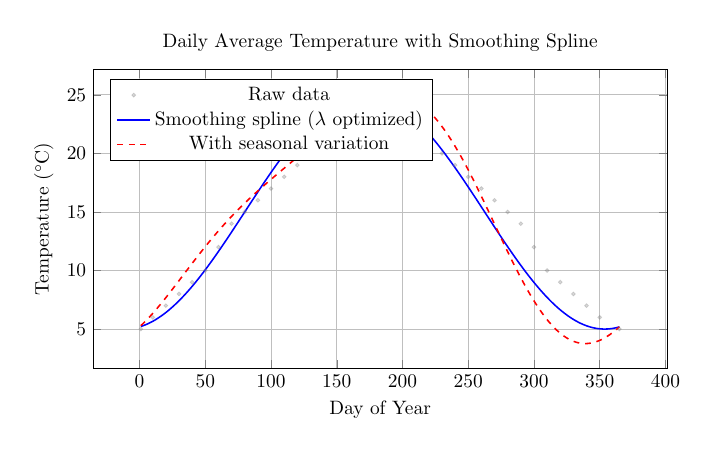
\begin{tikzpicture}[scale=0.7]
    \begin{axis}[
        width=12cm,
        height=7cm,
        xlabel={Day of Year},
        ylabel={Temperature ($^\circ$C)},
        title={Daily Average Temperature with Smoothing Spline},
        legend pos=north west,
        grid=major
    ]
    % Simulated daily temperature data
    \addplot[only marks, mark=*, mark size=1pt, gray, opacity=0.3] coordinates {
        (1, 5) (10, 6) (20, 7) (30, 8) (40, 9) (50, 10) (60, 12) (70, 14)
        (80, 15) (90, 16) (100, 17) (110, 18) (120, 19) (130, 20) (140, 21)
        (150, 22) (160, 23) (170, 24) (180, 25) (190, 24) (200, 23) (210, 22)
        (220, 21) (230, 20) (240, 19) (250, 18) (260, 17) (270, 16) (280, 15)
        (290, 14) (300, 12) (310, 10) (320, 9) (330, 8) (340, 7) (350, 6) (365, 5)
    };
    \addlegendentry{Raw data}
    
    % Smoothing spline fit (sine wave approximation)
    \addplot[domain=1:365, samples=200, thick, blue] {15 + 10*sin(deg((x-80)*2*pi/365))};
    \addlegendentry{Smoothing spline ($\lambda$ optimized)}
    
    % Seasonal pattern
    \addplot[domain=1:365, samples=200, thick, red, dashed] {15 + 10*sin(deg((x-80)*2*pi/365)) + 2*sin(deg(x*4*pi/365))};
    \addlegendentry{With seasonal variation}
    \end{axis}
\end{tikzpicture}

\begin{itemize}
    \item Captures annual temperature cycle
    \item Smooths out daily noise
    \item Reveals underlying seasonal pattern
\end{itemize}
\end{frame}

\begin{frame}{Applications}
\begin{block}{Time Series Analysis}
\begin{itemize}
    \item Trend extraction
    \item Seasonal decomposition
    \item Smoothing noisy measurements
\end{itemize}
\end{block}

\begin{block}{Regression}
\begin{itemize}
    \item Nonparametric regression
    \item Basis for GAMs
    \item Functional data analysis
\end{itemize}
\end{block}

\begin{block}{Data Visualization}
\begin{itemize}
    \item Smooth curve fitting
    \item Trend lines
    \item Exploratory data analysis
\end{itemize}
\end{block}
\end{frame}

\begin{frame}{Summary}
\begin{block}{Key Concepts}
\begin{itemize}
    \item Smoothing splines minimize: $\text{RSS} + \lambda \times \text{roughness}$
    \item Solution is a natural cubic spline with knots at data points
    \item Smoothing parameter $\lambda$ controls bias-variance trade-off
    \item Choose $\lambda$ via cross-validation (GCV)
    \item Effective degrees of freedom: $\text{df}_\lambda = \text{tr}(\mathbf{S}_\lambda)$
\end{itemize}
\end{block}

\begin{block}{Takeaways}
\begin{itemize}
    \item Automatic, flexible, and smooth
    \item Computationally efficient ($O(n)$)
    \item Foundation for GAMs and nonparametric regression
    \item Useful for exploratory analysis and visualization
\end{itemize}
\end{block}
\end{frame}

\begin{frame}{References and Further Reading}
\begin{itemize}
    \item Hastie, Tibshirani, Friedman. \textit{The Elements of Statistical Learning}, Chapter 5
    \item Green, Silverman. \textit{Nonparametric Regression and Generalized Linear Models}
    \item Wood, S. N. \textit{Generalized Additive Models: An Introduction with R}
    \item Reinsch, C. H. (1967). Smoothing by spline functions
\end{itemize}
\end{frame}

\end{document}

